\documentclass{beamer}
\usetheme[pageofpages=de,% String used between the current page and the
                         % total page count.
          bullet=circle,% Use circles instead of squares for bullets.
          titleline=true,% Show a line below the frame title.
          alternativetitlepage=true,% Use the fancy title page.
          titlepagelogo=../img/fse_ministerio_ancho_texto.png%,% Logo for the first page.
	  %watermark=junta_girado,
          %watermarkheight=75px,% Height of the watermark.
          %watermarkheightmult=4,% The watermark image is 4 times bigger
                                % than watermarkheight.
          ]{Torino}

\usepackage[spanish]{babel} % Para separar correctamente las palabras
\usepackage[utf8]{inputenc} % Este paquete permite poner acentos y eñes usando codificación utf-8

\usepackage{color}

\author{IES Gonzalo Nazareno\\
IES Los Albares\\
IES La Campiña\\
IES Ingeniero de la Cierva\\
\vspace{.5cm}

\includegraphics[width=0.2\textwidth]{cc_by_sa.png}}
\title{IaaS en educación}
\institute{Proyecto de Innovación\\ {\color{white} .\\} \emph{Implantación y
    puesta a punto de la infraestructura de un cloud computing privado para el
    despliegue de servicios en la nube}}  
\begin{document}
\begin{frame}[t,plain]
\titlepage
\end{frame}

\begin{frame}
  \frametitle{Cloud Computing}
\end{frame}

\begin{frame}
  \frametitle{Evolución metodológica}
  \begin{itemize}
  \item A la par de la evolución tecnológica, se ha producido una evolución en
    los métodos de enseñanza, que podríamos separar en 3 fases:
    \begin{itemize}
    \item Primera fase: Utilización de equipos físicos
    \item Segunda fase: Utilización de máquinas virtuales
    \item Tercera fase: Utilización de IaaS
    \end{itemize}
  \item Estas fases no son excluyentes: una fase siempre puede incluir las
    anteriores.
  \item Todas tienen ventajas e inconvenientes, pero la tercera fase ofrece
    escenarios imposibles de utilizar anteriormente.

  \end{itemize}
\end{frame}

\begin{frame}
  \frametitle{Evolución metodológica. Primera fase}
  \begin{columns}
    \column{.6\textwidth}
    \begin{itemize}
    \item Utilización de máquinas físicas
      \begin{itemize}
      \item Una máquina por alumno
      \item Algunos servidores compartidos
      \end{itemize}
      \item Pros:
      \begin{itemize}
      \item Fácil despliegue y puesta en marcha
      \end{itemize}
      \item Contras:
      \begin{itemize}
      \item Prácticas muy limitadas por número de equipos y tipo de
        configuraciones
      \item Hardware poco variado
      \item Prácticas muy ``académicas''
      \item Muchos tiempos muertos entre prácticas
      \end{itemize}
    \end{itemize}
    \column{.4\textwidth}
    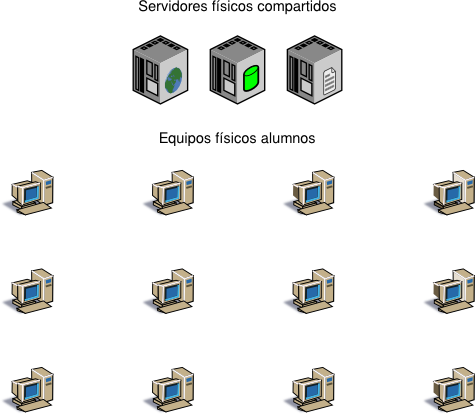
\includegraphics[width=\columnwidth]{../img/epoca1.png}
  \end{columns}
\end{frame}

\begin{frame}
  \frametitle{Evolución metodológica. Segunda fase}
  \begin{columns}
    \column{.6\textwidth}
    \begin{itemize}
    \item Utilización de máquinas virtuales
      \begin{itemize}
      \item Una máquina por alumno
      \item Varias máquinas virtuales por máquina física
      \end{itemize}
      \item Pros:
      \begin{itemize}
      \item Cada alumno dispone de un entorno ``completo'' e independiente
      \item Prácticas menos rígidas
      \item Se aprende virtualización de forma transversal
      \end{itemize}
      \item Contras:
      \begin{itemize}
      \item Entorno más complejo
      \item Equipos actualizados para los alumnos
      \end{itemize}
    \end{itemize}
    \column{.4\textwidth}
    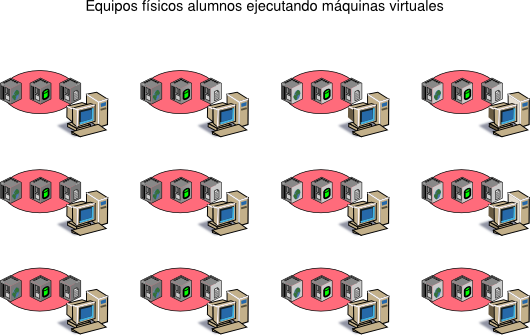
\includegraphics[width=\columnwidth]{../img/epoca2.png}
  \end{columns}
\end{frame}

\begin{frame}
  \frametitle{Evolución metodológica. Tercera fase}
  \begin{columns}
    \column{.6\textwidth}
    \begin{itemize}
    \item Utilización de IaaS
      \begin{itemize}
      \item Una máquina física por alumno
      \item IaaS privado de la organización
      \end{itemize}
      \item Pros:
      \begin{itemize}
      \item Enorme capacidad computacional
      \item Utilización de entornos preconfigurados
      \item Simulación de entornos reales complejos
      \item Equipos básicos para los alumnos
      \item Se aprende IaaS de forma transversal
      \end{itemize}
      \item Contras:
      \begin{itemize}
      \item Sistema muy centralizado
      \item Imprescindible administración del Cloud
      \item Inversión inicial importante
      \end{itemize}
    \end{itemize}
    \column{.4\textwidth}
    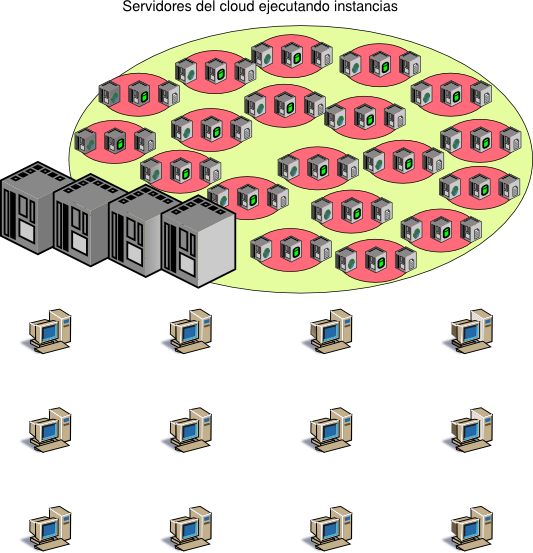
\includegraphics[width=\columnwidth]{../img/epoca3.png}
  \end{columns}
\end{frame}

\begin{frame}
  \frametitle{Nueva forma de aprendizaje}
  \begin{itemize}
  \item La utilización de IaaS en el ámbito académico conlleva una nueva forma
    de aprender
  \item Con el uso de MVs se había impuesto una forma de aprender que no era
    siempre la mejor, por ejemplo:
    \begin{itemize}
    \item Para utilizar un SGBD había que instalarlo y configurarlo antes
    \item Para desplegar una aplicación web, había que configurar previamente
      todo el servidor de aplicaciones
    \item Para hacer prácticas de ZFS había que instalar Solaris o FreeBSD
    \end{itemize}
    \item Un IaaS puede contar con gran cantidad de imágenes preconfiguradas de
      sistemas con muy diversas configuraciones $\Rightarrow$ La forma de
      aprender no viene condicionada por la necesidad de una configuración previa:
      \begin{itemize}
      \item Primero se utiliza el SGBD
      \item Posteriormente, cuando sea oportuno, se aprende a instalarlo y
        configurarlo
      \end{itemize}

  \end{itemize}
\end{frame}

\begin{frame}
  \frametitle{Escenarios (II)}
  \begin{description}
  \item[Instalación y configuración de un servicio]
  \end{description}
  Los pasos típicos a seguir serían:
  \begin{itemize}
  \item Cada alumno inicia una instancia del SO en el que va a instalar el
    servicio (no es necesario que previamente sepa instalar ese SO).
  \item Realiza la instalación del servicio
  \item Realiza la configuración del servicio. Si esta configuración dura
    más de una clase, suspende la instancia y la reinicia en la siguiente
    clase.
  \item Una vez terminada la configuración puede crear una instantánea para
    utilizarla como base en posteriores prácticas.
  \item Si algún alumno no ha podido realizar la configuración correctamente
    podrá utilizar la instantánea de un compañero en clases posteriores.
  \end{itemize}
\end{frame}
\end{document}
